\documentclass[professionalfonts]{beamer}
\newif\ifanswers
%\answerstrue % comment out to hide answers
\answersfalse
\usepackage[familydefault,light]{Chivo} 
\usepackage[T1]{fontenc}
\usenavigationsymbolstemplate{}
\usepackage[]{hyperref}
\usepackage{tikz,pgf,pgfarrows,pgfnodes,pgfbaseimage}
\graphicspath{{./Pics/}}
\usetikzlibrary{shapes}
\usepackage{setspace}
\newcommand{\evi}[1]{{\colorbox{yellow!50}{{#1}}}}
\newcommand{\exe}[1]{{\color{black!50}{{#1}}}}
\newcommand{\kw}[1]{{\colorbox{black!30}{\color{white}{#1}}}}
\tikzstyle{nd}=[circle,draw=black,thick,minimum size=.8cm,inner sep=1pt]
\setbeamercovered{transparent}
\usetheme{Singapore}
\tikzstyle{nodo}=[ellipse,draw=black!60,fill=black!10,line width=.7pt,minimum width=.7cm,minimum height=.4cm]
\usecolortheme[named=gray]{structure}
\setbeamercolor{block title}{bg=black!20,fg=black}
\setbeamercolor{block body}{bg=black!10,fg=black}

\ifanswers
\title{Algoritmi Numerici (Parte I)}
\subtitle{[Esercitazione 1] Numeri Naturali $\mathbb{N}$, \\Algoritmo di Horner e suo Inverso}
\else
\title{Numerics (Part I)}
\subtitle{[Exercise Session 1] Natural Numbers $\mathbb{N}$, \\Horner's Algorithm, Inverse}
\fi
\date{}
\author{Alessandro Antonucci\\{\tt alessandro.antonucci@supsi.ch}}
%%%%%%%%%%%%%%%%%%%%%%%%%%%%
%\setstretch{1.4}
\begin{document}
\maketitle

\frame{\frametitle{\ifanswers Da base $b$ a base $10$ \else From base $m$ to base $10$ \fi} 
\begin{columns}
\begin{column}[T]{0.5\textwidth}
\Large\centering
$100110111_2 = 311_{10}$
\vskip 2mm
$200102_3 = 497_{10}$
\vskip 2mm
$2177_8 = 1151_{10}$
\end{column}
\begin{column}[T]{0.5\textwidth}
\Large\centering
$AC12_{16} = 44050_{10}$
\vskip 2mm
$1111_3 = 40_{10}$
\vskip 2mm
$1111_4 = 85_{10}$
\end{column}
\end{columns}
\vskip 10mm
\centering
\ifanswers Nota: un numero in base $b$ usa le cifre \else Digits used for base $b$ numbers are \fi   $\{ 0 , 1 , 2 , \ldots , b-1 \}$ 
\vskip 2mm
\ifanswers 
Se $b>10$ servono altri simboli  (es. lettere) \\ Esadecimale $b=16$:
\else
For $b>10$ we need more symbols  (ex. letters) \\ Hexadecimal  $b=16$:

\fi
\vskip 2mm
\begin{center}
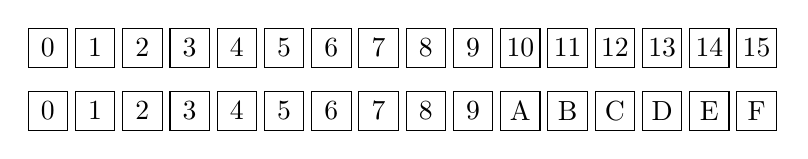
\begin{tikzpicture}
	\foreach \x in {0,1,2,3,4,5,6,7,8,9,10,11,12,13,14,15}
	\draw (\x*0.6,0) +(-.25,-.25) rectangle ++(.25,.25);
	\foreach \x in {0,1,2,3,4,5,6,7,8,9,10,11,12,13,14,15}
	\draw (\x*0.6,0) node{\x};
	\foreach \x in {0,1,2,3,4,5,6,7,8,9,10,11,12,13,14,15}
	\draw (\x*0.6,-.8) +(-.25,-.25) rectangle ++(.25,.25);
	%\foreach \x in {0,1,2,3,4,5,6,7,8,9,10,11,12,13,14,15}
	\foreach \x in {0,1,2,3,4,5,6,7,8,9}
	\draw (\x*0.6,-.8) node{\x};
	\draw (10*0.6,-.8) node{A};
	\draw (11*0.6,-.8) node{B};
	\draw (12*0.6,-.8) node{C};
	\draw (13*0.6,-.8) node{D};
	\draw (14*0.6,-.8) node{E};
	\draw (15*0.6,-.8) node{F};
\end{tikzpicture}
\end{center}}

\frame{\frametitle{\ifanswers Da base 10 a base n \else From base 10 to base n\fi}
\begin{columns}
\begin{column}[T]{0.5\textwidth}
\Large\centering
$2143_{10} =100001011111_{2}$
\vskip 2mm
$13458_{10} = 3492_{16}$
\vskip 2mm
$798_{10} = 1436_{8}$
\end{column}
\begin{column}[T]{0.5\textwidth}
\Large\centering
$144_{10} = 10010000_{2}$
\vskip 2mm
$144_{10} = 12100_{3}$
\vskip 2mm
$144_{10} = 2100_{4}$
\end{column}
\end{columns}
}
\frame{\frametitle{\ifanswers Da base m a base n \else From base m to base n\fi}
\begin{center}
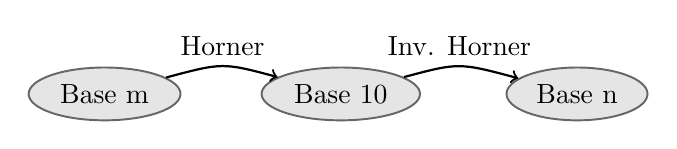
\begin{tikzpicture}
\node[nodo] (a)  at (0,0) {Base m};
\node[nodo] (b)  at (3,0) {Base 10};
\node[nodo] (c)  at (6,0) {Base n};
\draw[->,above,thick] (a) .. controls (1.5,.4) ..  (b) node[midway] {Horner};
\draw[->,above,thick] (b) .. controls (4.5,.4) ..  (c) node[midway] {Inv. Horner};
%\draw[->,below,thick] (d) .. controls (2.5,-.4) .. (b) node[midway] {Inverso};
\end{tikzpicture}
\end{center}
\begin{itemize}\Large
	\item $1032_4 = 78_{10} = 2220_{3}$
	\item $101101_2 = 45_{10} = 140_{5}$
	\item $2177_8 = 1151_{10} = 47F_{16}$
\end{itemize}
}
\frame{\frametitle{\ifanswers Da base m a base n  (trasformazioni dirette)\else From base m to base n (direct transformations)\fi}
\Large
$210745_{10}=\ldots_{100}?$
\vskip 2mm
$2 \cdot 10^5 +1 \cdot 10^4 +0 \cdot 10^3 + 7 \cdot 10^2 + 4 \cdot 10^1 + 5 \cdot 10^0=$
\vskip 2mm
$21 \cdot 100^2 + 7 \cdot 100^1 + 45 \cdot 100^0 $
\vskip 2mm
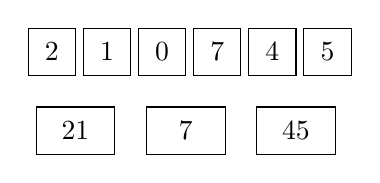
\begin{tikzpicture}
	\draw (0,0) +(-.3,-.3) rectangle ++(.3,.3);
	\draw (.7,0) +(-.3,-.3) rectangle ++(.3,.3);
	\draw (1.4,0) +(-.3,-.3) rectangle ++(.3,.3);
	\draw (2.1,0) +(-.3,-.3) rectangle ++(.3,.3);
	\draw (2.8,0) +(-.3,-.3) rectangle ++(.3,.3);
	\draw (3.5,0) +(-.3,-.3) rectangle ++(.3,.3);
	\draw (.3,-1) +(-.5,-.3) rectangle ++(.5,.3);
	\draw (1.7,-1) +(-.5,-.3) rectangle ++(.5,.3);
	\draw (3.1,-1) +(-.5,-.3) rectangle ++(.5,.3);
	\draw (0,0) node{2};
	\draw (.7,0) node{1};
	\draw (1.4,0) node{0};
	\draw (2.1,0) node{7};
	\draw (2.8,0) node{4};
	\draw (3.5,0) node{5};
	\draw (.3,-1) node{21};
	\draw (1.7,-1) node{7};
	\draw (3.1,-1) node{45};
\end{tikzpicture}
\vskip 2mm
$100 = 10^2$: \ifanswers cifre raggruppate a due a due \else grouping digits two-by-two\fi
\vskip 3mm
 \ifanswers Stessa cosa se \else Just the same for \fi  $b\neq 10$ 
}
\frame{\frametitle{\ifanswers Trasformazioni Dirette \else Direct Transformations \fi}
\begin{itemize}\Large
	\item $1032_4 = 1001110_{2}$
	\item $101101_2 = 2D_{16}$
	\item $2177_8 = 010001111111_{2}$
\end{itemize}}

\frame{\frametitle{\ifanswers Esercizio \else Exercise \fi \# 1}
\Large
\begin{itemize}
\item $2177_8=\ldots_2${\small$\color{black!20}{(=1151_{10}=10001111111_2})$}
\item $10220_3=\ldots_9${\small$\color{black!20}{(=105_{10}=126_9})$}
\item $20016_7=\ldots_5${\small$\color{black!20}{(=4815_{10}=123230_5})$}
\item $AC12_{16}=\ldots_8${\small$\color{black!20}{(=44050_{10}=126022_8})$}

\end{itemize}}

\frame{\frametitle{\ifanswers Esercizio \else Exercise \fi \# 2}
\begin{itemize}
\item $1111_2=\color{black!20}{15_{10}}$, $11111_2=\color{black!20}{31_{10}}$, $111111_2=\color{black!20}{63_{10}}$ 
\item $222_3=\color{black!20}{26_{10}}$, $2222_3=\color{black!20}{80_{10}}$, $22222_3=\color{black!20}{242_{10}}$, 
\item $44_5=\color{black!20}{24_{10}}$, $444_5=\color{black!20}{124_{10}}$, $4444_5=\color{black!20}{624_{10}}$, 
\vskip 10mm
\begin{center}
${\underbrace{bbbb \ldots bb_{b+1}}_{\text{n cifre}}}=(b+1)^n-1$%{b+1}$%% = \ldots_{10}$
\end{center}
\end{itemize}}

\frame{\frametitle{\ifanswers Esercizio \else Exercise \fi \# 3}
\setstretch{1.2}
\normalsize
\ifanswers
In C una variabile {\tt unsigned int} richiede al compilatore di allocare 32 bit, che verranno utilizzati per rappresentare numeri interi senza segno secondo le regole del sistema posizionale in base due
\vskip 1mm
{\tt unsigned short/long} fanno lo stesso con 16/64 bit. 
\else
For the C language a {\tt unsigned int} variables ask the compiler to allocate 32 bits, to be used to represent unsigned integer numbers according to the positional numeral system in base 2.
\vskip 1mm
Formats {\tt unsigned short/long} are doing the same with 16/64 bits
\fi
\small
\begin{itemize}
\item \ifanswers Rappresentare il numero 131'086 nei tre formati compattando le sequenze di bit in esadecimale \else Find the bit representation of the number 131'086 in the three formats and compact the sequences of bits in hexadecimal \fi
\item \ifanswers Fare lo stesso per il pi\`u grande numero di ogni formato \else Do the same for the largest number of each format \fi
\item \ifanswers Leggere le sequenze esadecimali con l'algoritmo di Horner\else Read the hexadecimal sequences with Horner's algorithm \fi
\begin{center}
$A019$ $\color{black!20}{(=40985_{10}})$ {\tt unsigned short}\\
$010C|7142$ $\color{black!20}{(=17592642_{10})}$ {\tt unsigned int}\\
$0000|100A|0007|3501$ $\color{black!20}{(\simeq 1.765 \cdot 10^{13})}$ {\tt unsigned long}\\
\end{center}
\end{itemize}}
\end{document}
